\chapter[Pulse signal preprocessing]{\uppercase{Pulse signal preprocessing}}
\label{chap:three}

Owing to the electromagnetic interference in surrounding environment,
high frequency noise will be superimposed on the original signal
amid collection, affecting the signal analysis. 
Meanwhile, the breathing or body movement of participant will also
cause the signal baseline drift. Distortion of pulse features
extracted would probably occur afterwards unless the baseline drift problem
was solved. Therefore, the both problems must be properly handled
towards the original pulse signal. In addition, since the subsequent
pulse feature extraction is based on a single period of pulse
waveform, a period segmentation algorithm fulfills the task to split
signal series. The chapter employs wavelet transform to filter
high-frequency noise, wavelet-based cascaded adaptive filter to remove
baseline drift, and a period detection algorithm to divide periods.
At last, the pulse waveform is normalized.
Figure~\ref{fig:preprocessing} demonstrates the outline of this
chapter.
\begin{figure}[htpb]
    \begin{center}
        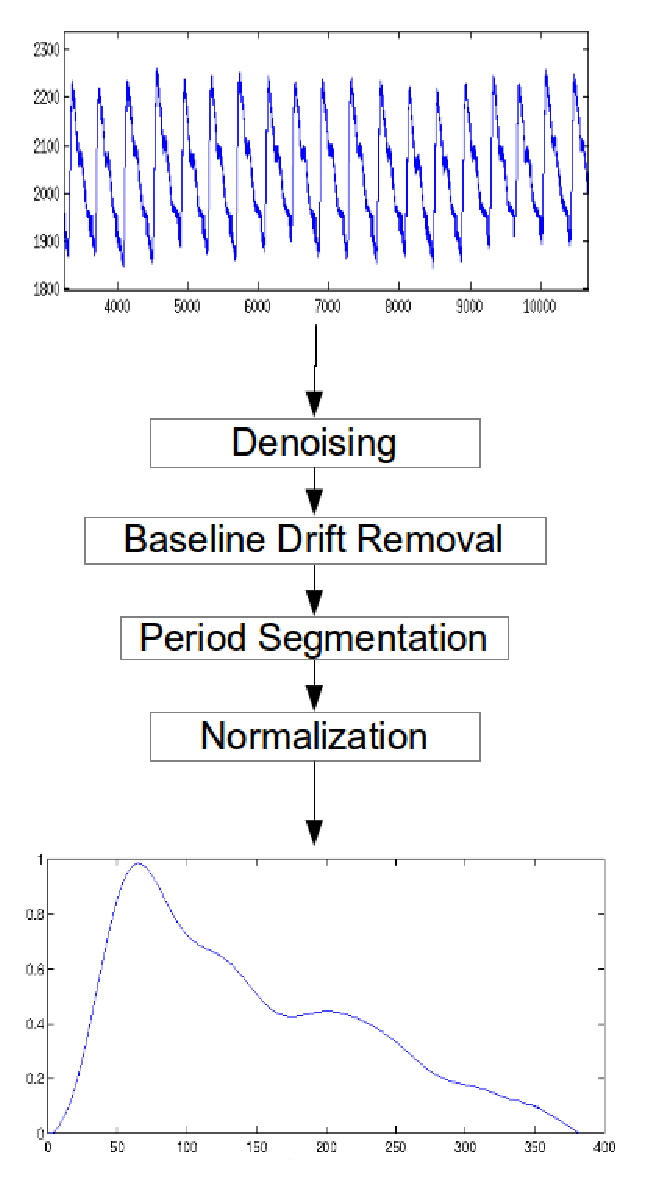
\includegraphics[width=0.4\textwidth]{preprocessing}
    \end{center}
    \caption{Preprocessing procedures}
    \label{fig:preprocessing}
\end{figure}



\section{Burring}
The human wrist pulse signal is a weak physiological signal that
is susceptibly to high-frequency noise caused by interference of
electromagnetic devices. This sort is called \emph{burr} because the
noise looks like small notches in the fringe of objects. See
Figure~\ref{fig:beforeburr}. 
\begin{figure}[htpb]
    \begin{center}
        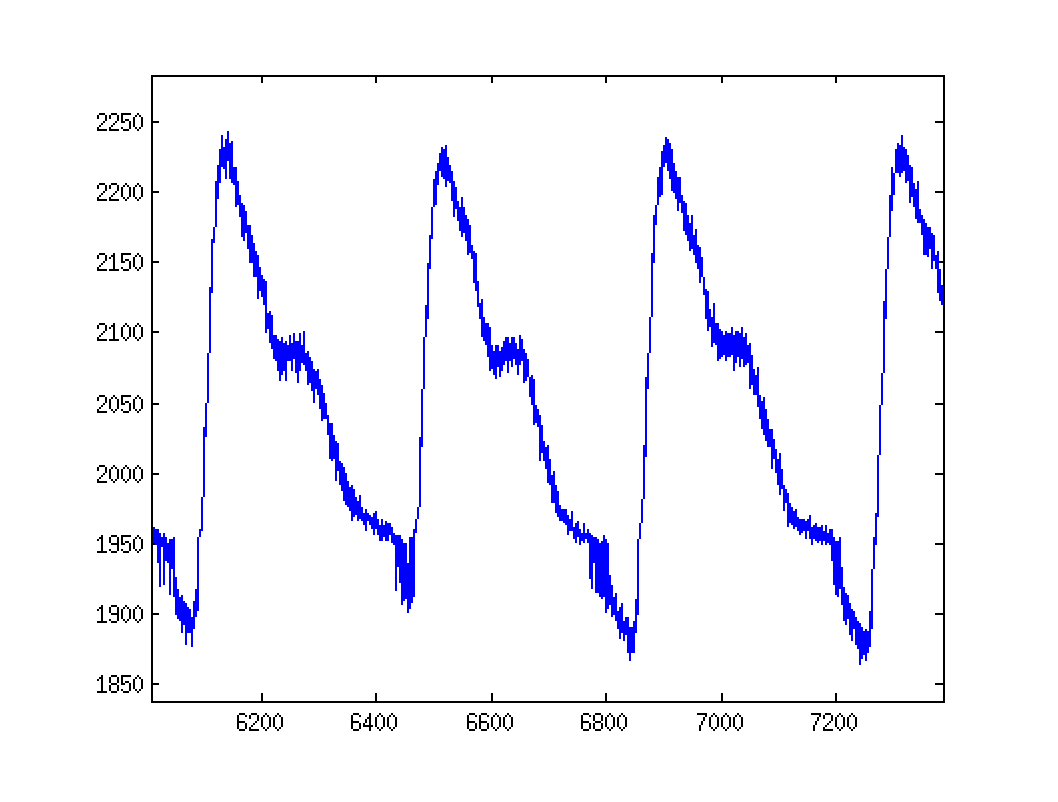
\includegraphics[width=0.7\textwidth]{beforeburr}
    \end{center}
    \caption{Pulse signal with burr noise}
    \label{fig:beforeburr}
\end{figure}
By careful observation, the burrs in pulse signals present a jagged
form in overall, which means glitches float uniformly around the real
value. In actual processing, the majority of signals may contain
spikes or mutation, and the noise signal is not stable white noise yet. 
So does the pulse signal. Fourier transform based spectral analysis is
the dominant analytical tool for frequency 
domain analysis. However, Fourier transform cannot provide any
information of the spectrum changes with respect to time.  Fourier
transform assumes the signal is stationary, but pulse signal is always
non-stationary. The traditional Fourier transform 
considers information merely on frequency-domain and becomes powerless
to differentiate the change on a specific point. Admittedly, the
traditional Fourier low pass filter could suppress the noise, it
meanwhile blurs the noisy edge of one-dimension signal. If the
low-pass frequency range is narrow, high-frequency components of the
mutation part will be treated as noise to be filtered,
which led to a certain amount of distortion in the mutation part; If
the range of low-pass frequency is set too wide, the noise may not be
effectively filtered out. To overcome this deficiency, a modified method-short
time Fourier transform allows to represent the signal in both time and
frequency domain through time windowing function. The window
length determines a constant time and frequency resolution. Thus, a
shorter time windowing is used in order to capture the transient
behavior of a signal; we sacrifice the frequency resolution.
So, an alternative mathematical tool- wavelet
transform must be selected to extract the relevant time-amplitude
information from a signal.  In the meantime, we can improve the signal to noise ratio based on
prior knowledge of the signal characteristics. 

\subsection{Wavelet-based denoising}
Wavelet transform is a inheritance and development of Fourier
transform, that not only has a profound and comprehensive theory, 
but also emerges its wider application prospect. As is known to
everyone, a $\Psi(t)$ is called a \emph{Mother Wavelet} if it meets
the following condition: 
\begin{equation}
    C_\Psi=\int_R \frac{|\Psi(\omega)|^2}{|\omega|}\mathrm{d}\omega <
    \infty, \quad \mathrm{for} \; \Psi \in L^2(R)
    \label{waveletdefinition}
\end{equation}
Do a scaling and shifting operation to the mother function as 
\begin{equation}
    \Psi_{a,b}(t) = |a|^{-\frac{1}{2}}\Psi(\frac{t-b}{a}), \quad b \in
    R, \, a \in R - \{0\}.
    \label{waveletbase}
\end{equation}
Then The function family ${\Psi_{a,b}(t)}$ is called \emph{wavelet base},
where $a$ is the scale parameter and $b$ is the shift parameter. If
$a=2^j,b=k\cdot 2^j,\,j,k \in Z$, then
\begin{equation}
    \Psi_{j,k}(t)=2^{-\frac{j}{2}}\Psi(2^{-j}t-k).
    \label{wavelet3}
\end{equation}
If $\Psi(t)$ is properly chosen, ${\Psi_{j,k}(t)}$ could consist of a
family of orthonormal wavelet bases. So any function $f(t)\in L^2(R)$ can
be expanded in the form of orthonormal wavelet series:
\begin{equation}
    f(t)=\sum_{j,k=-\infty}^{+\infty} c_{j,k}\Psi_{j,k}(t)
    \label{waveletdecomp}
\end{equation}
where $c_{j,k}=<f,\Psi_{j,k}>$. The important information of signal
$f(t)$ disperses into each layer. It helps people handle specifics of
signals more conveniently from both time and space. 

One important application of wavelet transform is signal denoising.
The wavelet can efficiently remove noise on account of its good 
locality in both time-domain and frequency-domain. It could 
distinguish the mutation part and noise of signals and successfully
achieve the elimination of noise for non-stationary signals. In
essence, the wavelet transform carries out the function to depress the
useless part of the signal and intensify the useful part at the same
time.~\cite{debnath2002wavelet, Changfa2001, Qiwen2001}. 

Therefore, the paper will give priority to employ the one-dimension
wavelet transform to smooth the pulse signal. The wavelet
transform denoising process usually is divided into 3 steps~\cite{polikarwavelet}:
\begin{enumerate}[(1)]
    \item Apply wavelet transform to the noisy signal to produce the
        noisy wavelet coefficients to the level which we can properly
        distinguish the PD occurrence.
    \item Select appropriate threshold limit at each level and
        threshold method (hard or soft thresholding) to best remove
        the noises.
    \item Inverse wavelet transform of the thresholded wavelet
        coefficients to obtain a denoised signal. 
\end{enumerate}
Of the three steps, the most critical point is how to choose the
threshold and the corresponding quantification. To some extent, it
has a bearing on the effect of signal denoising. The detailed denosing
process based on wavelet transform aiming at pulse signal is shown as
below: 
\subsubsection{Wavelet selection}
Wavelet transform is essentially a description of signal features within
the space composed of a group of wavelet mother functions. The mother
function plays a critical role in wavelet transform. To best
characterize the spikes in a noisy signal, we should select our
``mother wavelet'' carefully to better approximate and capture the
transient spikes of the original signal. ``Mother wavelet'' will not
only determine how well we estimate the original signal in terms of
the shape of the PD spikes, but also, it will affect the frequency
spectrum of the denoised signal. There are seven factors needed to
consider for better choice\cite{xin2003fan}. 
\begin{enumerate}[(1)]
    \item Regularity. It is very important to obtain a smoother effect
        for reconstruction of the signal. Generally speaking, the
        more orthogonal, the better denoising effect it will reach.
    \item Compact support and attenuation. These are two important
        attributes of wavelet. In general, a wavelet will have a
        better localization capacity if it attenuates quicker. And the
        compact support of wavelet base is expected in time-domain.
    \item Symmetry. Symmetric or antisymmetric scaling function and
        wavelet function could construct compactly supported
        orthogonal wavelet base with linear phase characteristic. 
    \item Vanishing moment property. In most situations it is useful
        to restrict $\Psi$ to be a continuous function with a higher number
        $M$ of vanishing moments, i.e. for all integer $m<M$
        \begin{equation}
            \int_R t^m \Psi(t) \mathrm{d}t=0
            \label{waveletvanish}
        \end{equation} 
        It has been proved that a wavelet with high enough vanishing
        moment could effectively detect the singular point.
    \item The time-frequency window and its area. The smaller the
        window size is, the stronger the localization capacity is
        achieved. Since the time-domain window and frequency-domain
        window is resizable, the wavelet could analyze signals adaptively. 
    \item Linear phase property. Linear phase is a property of a filter, where
        the phase response of the filter is a linear function of
        frequency, excluding the possibility of wraps at $\pm\pi$. 
        In signal processing, the scaling function and wavelet can be
        thought of as filter function since a filter with linear phase
        property or generalized linear phase at least is able to avoid
        the distortion during decomposition and reconstruction. 
\end{enumerate}

On consideration of the wavelet features above and the periodicity,
the paper chooses wavelet base $sym8$ as the filter. 

\subsubsection{Level of decomposition}
From the previous section, we have known the wavelet transform is
constituted by different levels. The maximum level to apply the
wavelet transform depends on how
many data points contain in a data set, since there is a down-sampling by 2 operation
from one level to the next one. In general, there is no solid criteria.
However, the following formula helps quickly decide the
number of decomposition level~\cite{liu2004compression}:
\begin{equation}
    J=int[log_2(f_s / f_f) -1]
    \label{waveletlevel}
\end{equation}
where $f_s$ denotes the sampling frequency (500Hz in this paper),  
$f_f$ denotes the fundamental frequency (within 10Hz in this paper),
and $int$ indicates to choose round number. Consequently, 5 levels
would be proper. 

\subsubsection{Threshold limits and denoised result}
The choice of the threshold is a
very delicate and important statistical problem.  On the one hand, a
big threshold leads to a large bias of the estimator. But on the other
hand, a small threshold increases the variance of the smoother.
Many methods for setting the threshold have been proposed. The most time-consuming
way is to set the threshold limit on a case-by-case basis. The limit
is selected such that satisfactory noise removal is achieved. But in
order to achieve a better denosing effect, it had better try different
cases of thresholds. There are usually three types of threshold. 
\begin{enumerate}[(1)]
    \item Hard thresholding. For one-dimension signal, the empirical
        threshold is calculated as 
        \begin{equation}
            t=sqrt{2\sigma^2 log(n)/n}
            \label{wavelethardthreshold}
        \end{equation}
        where $n$ is the length of the input signal and $\sigma^2$ is
        the variance of the noise. The variance of the noise is
        estimated based on the data. It is done by averaging the
        squares of the empirical wavelet coefficients at the highest
        resolution scale. Hard thresholding sets any coefficient less
        than or equal to the threshold to zero. 
    \item Soft thresholding. The only difference between the hard and
        the soft thresholding procedures is in the choice of the
        nonlinear transform on the empirical wavelet coefficients. For
        soft thresholding the following nonlinear transform is used: 
        \begin{equation}
            S(x)=\mathrm{sign}(x)(|x|-t)I(|x|-t),
            \label{waveletsoftthreshold}
        \end{equation}
        where $t$ is a threshold.  Adaptive thresholding.The threshold
        is subtracted from any coefficient that is greater than the
        threshold. This moves the time series toward zero. 
    \item Adaptive thresholding. The threshold selection rule is based on
        Stein's unbiased estimate of risk(quadratic loss function).
        One gets an estimate of the risk for a particular threshold
        value $(t)$. Minimizing the risks in $(t)$ gives a selection
        for the threshold value.
\end{enumerate}

The Figure~\ref{fig:threshold} shows the comparison of denoised
signals using the three thresholds described above. From the figures,
the soft thresholding method efficiently removes the high frequency
noise and preserves the original useful information; The hard
thresholding method still leaves out much noise not filtered; The
Adaptive thresholding method fails to work properly, probably in
account for its unsuitable application for this kind of noise.
\begin{figure}
  \centering
  \subfloat[The denoised signal using hard
  threshold]{\label{fig:hard}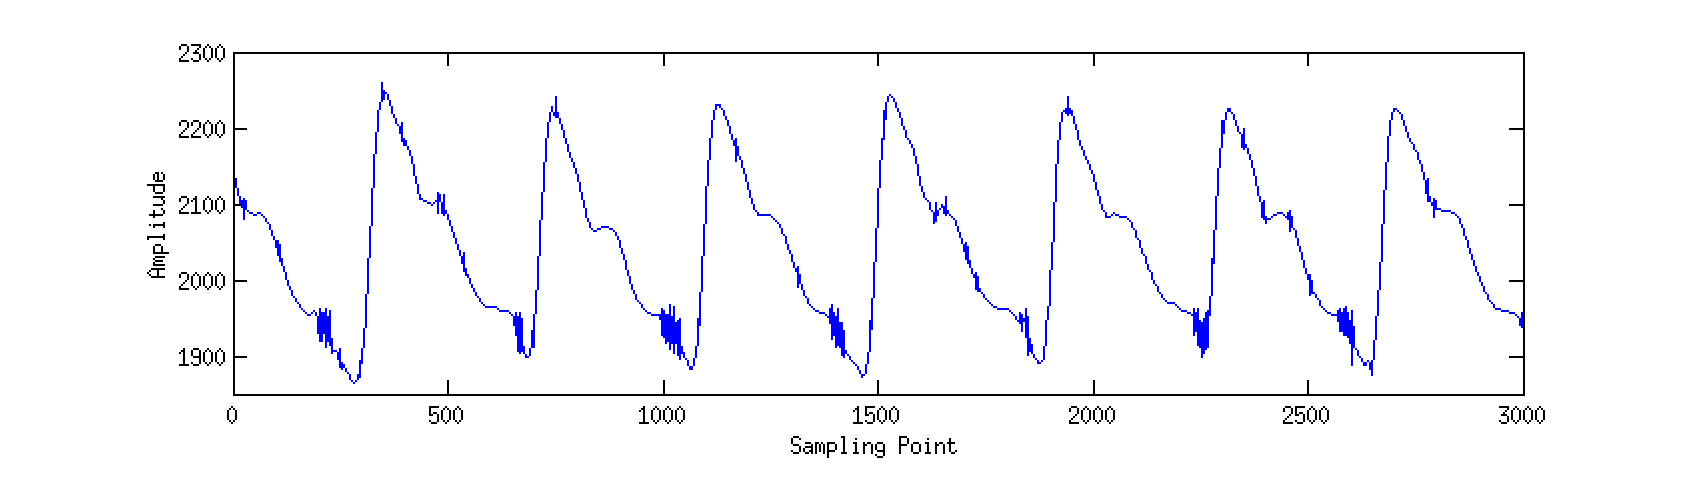
\includegraphics[width=0.9\textwidth]{hard}}\\
  \subfloat[The denoised signal using soft
  threshold]{\label{fig:soft}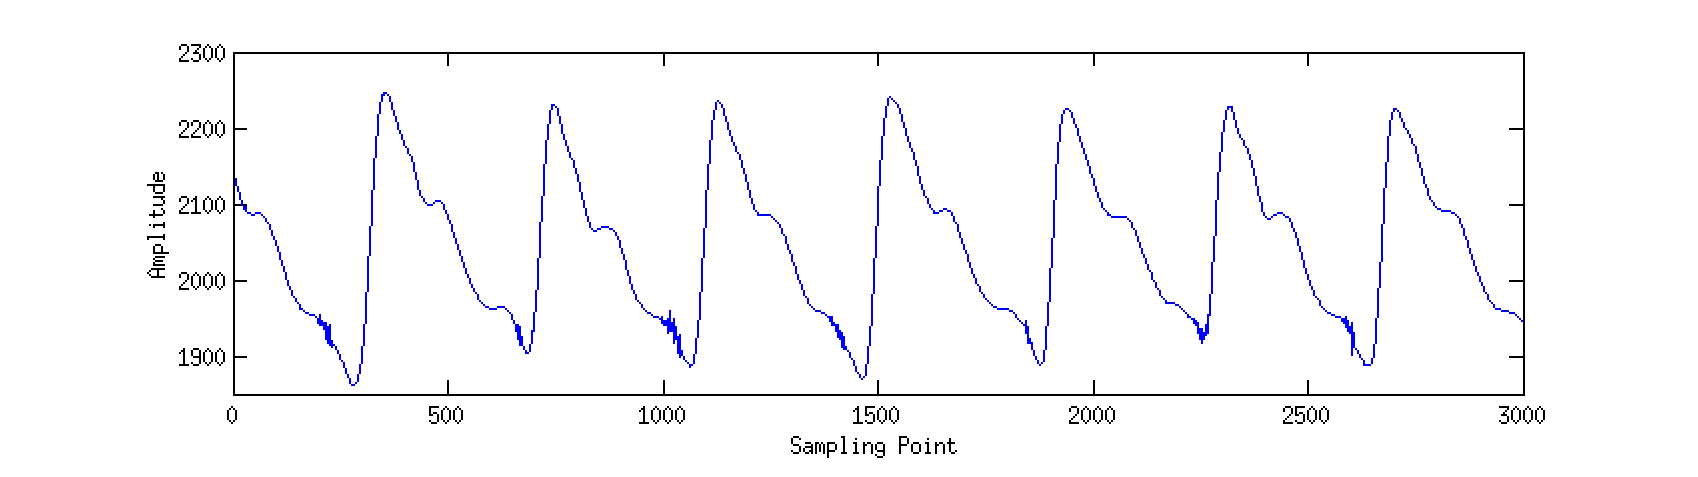
\includegraphics[width=0.9\textwidth]{soft}}\\
  \subfloat[The denoised signal using adaptive
  threshold]{\label{fig:adaptive}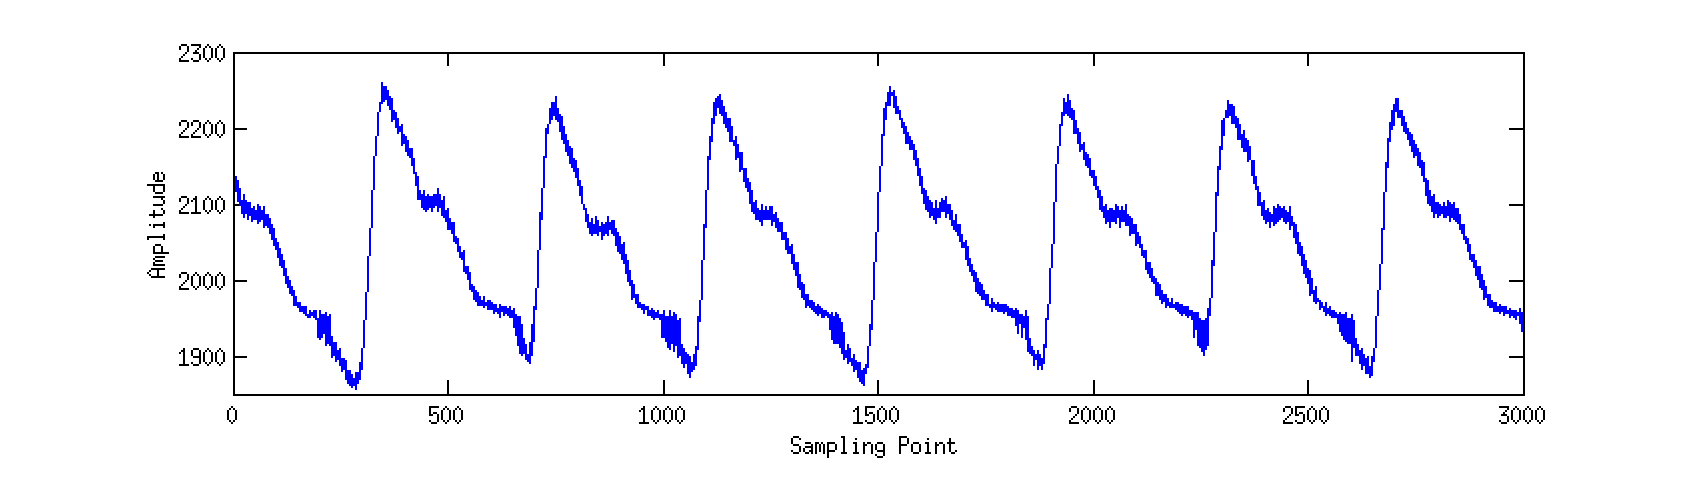
\includegraphics[width=0.9\textwidth]{adaptive}}\\
  \caption{The comparison of denoising effect with different thresholds}
  \label{fig:threshold}
\end{figure}

\subsection{Removal of electric power noise}
In carefully inspection to Figure~\ref{fig:soft}, it is found 
noise remaining in the tail of a period. So the frequency spectrum shown in
Figure~\ref{fig:powerfreqspec} shows the frequency distribution of noise.
The signal not only contains the electric power 50Hz noise, but also
noises higher than 50Hz from the internal system. 
The spike with frequency greater than 50Hz must be a burr noise since
the human pulse signal distributes below 15Hz.~\cite{wei1985frequency}
Hence, it is justified to remove all the noises upper than 50Hz.
So a low-pass linear filter is designed to filter them. 

Digital filters are typically considered in two categories: infinite impulse
response (IIR) and finite impulse response (FIR). FIR has two useful
properties which make it preferable to an IIR filter in this
experiment: inherent stability and linear phase. Linear phase implies an
important attribute because the pulse signal is a phase-sensitive
application. Although the disadvantage of FIR filters is that considerably more
computation power in a general purpose processor is required compared
to an IIR filter with similar sharpness or selectivity, properly
designed coefficients make FIR filters approximately as efficient as
IIR for many applications. 

The FIR filter is designed as these arguments: 
\begin{table}
    \centering
    \begin{tabular}{cc}
        Response type & Lowpass \\ \hline
        Design method & Kaiser Window \\ \hline
        Filter order & Minimum \\ \hline
        Frequency Specifications & $F_pass=48Hz, F_stop=50Hz$ \\ \hline
        Magnitude Specifications & $A_pass=1db, A_stop=80db$ \\\hline
    \end{tabular}
    \caption{The filter specifications}
    \label{tab:filter}
\end{table}
The magnitude response of the FIR filter under these arguments is
shown in Figure~\ref{fig:magnitutde}. By convolution filtering, the
noise with frequency higher than 50Hz is highly depressed.
Figure~\ref{fig:afterpower} gives the final pulse signal denoised. 
\begin{figure}[htpb]
    \begin{center}
        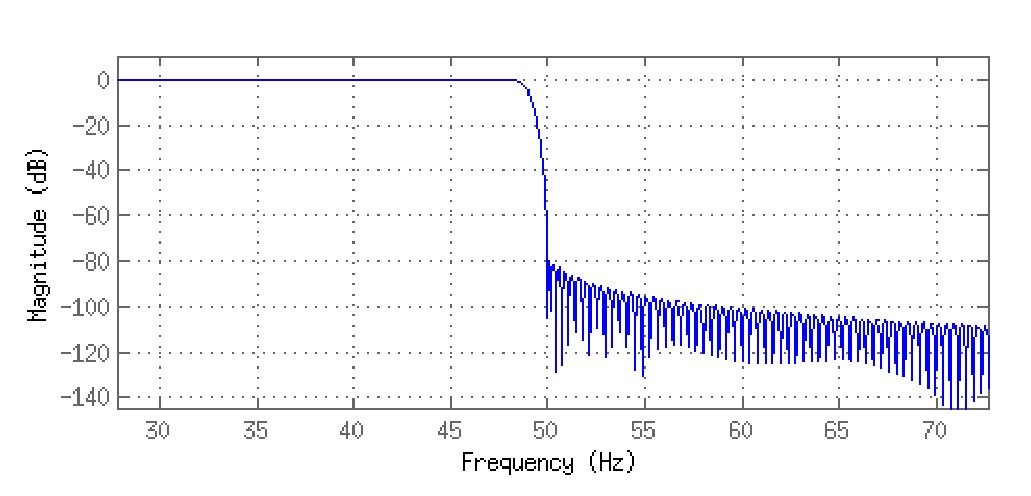
\includegraphics[width=0.7\textwidth]{filter}
    \end{center}
    \caption{Magnitude response of FIR filter}
    \label{fig:magnitutde}
\end{figure}

\begin{figure}
    \centering
    \subfloat[Pulse wave with power electric
    noise]{\label{fig:powernoise}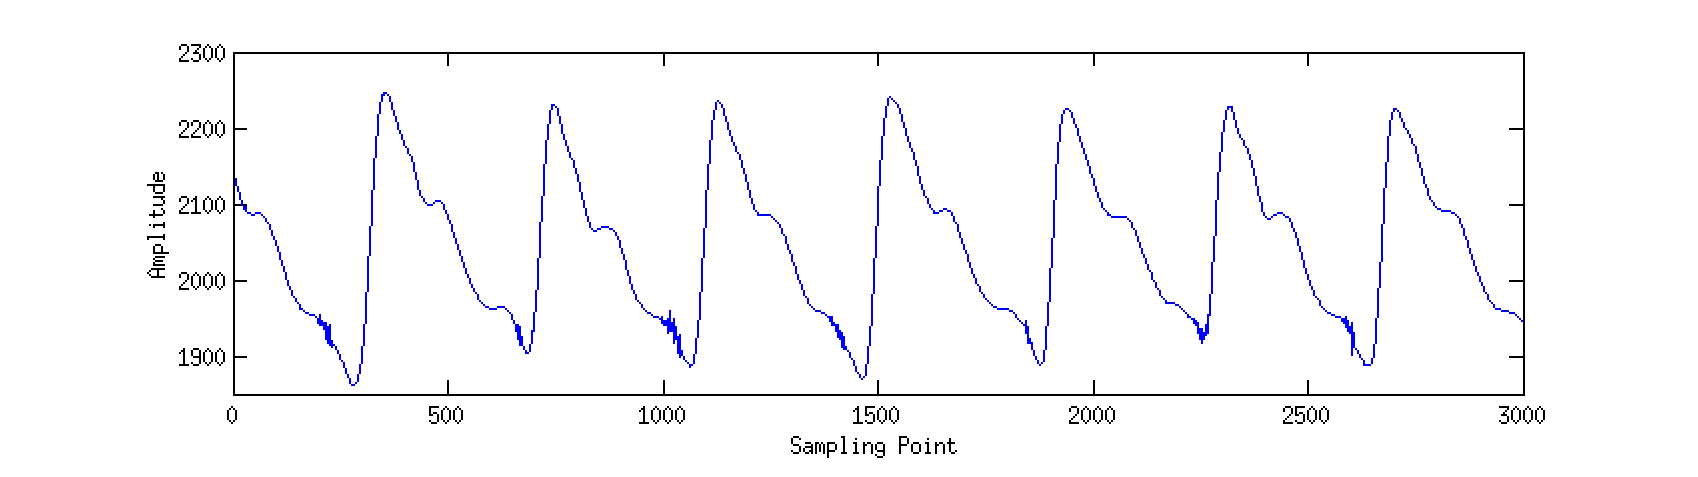
\includegraphics[width=0.7\textwidth]{soft}}\\
    \subfloat[The frequency
    spectrum]{\label{fig:powerfreqspec}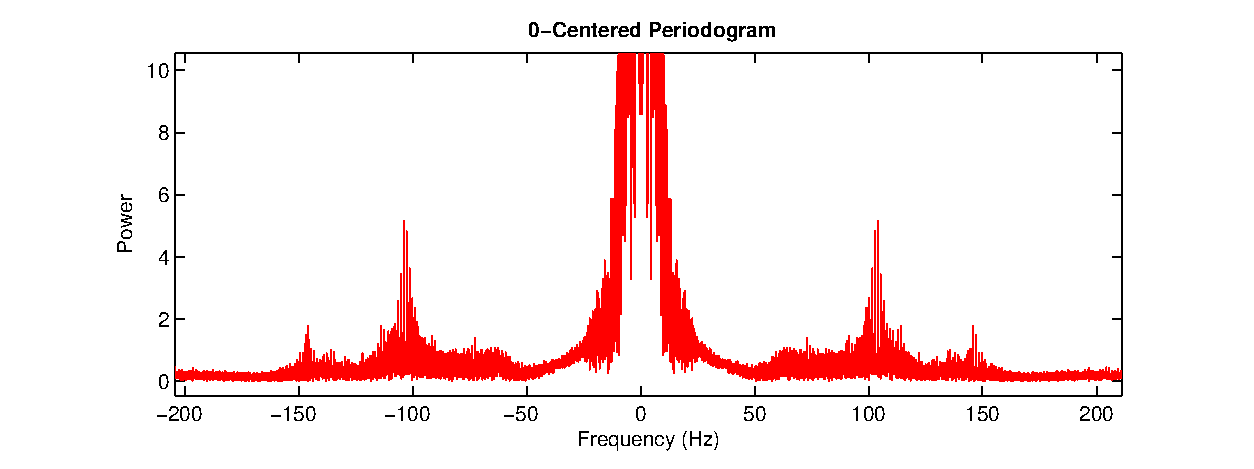
\includegraphics[width=0.7\textwidth]{50hz}}
    \caption{The pulse waveform before power noise removal}
    \label{fig:beforepower}
\end{figure}
\begin{figure}
    \centering
    \subfloat[Pulse wave after power electric noise
    removal]{\label{fig:nopowernoise}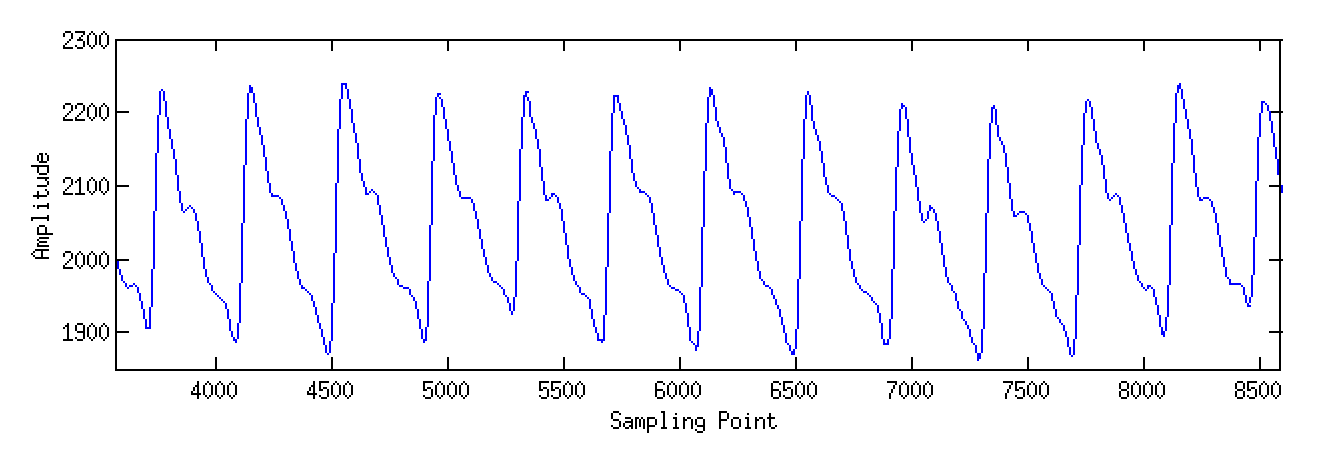
\includegraphics[width=0.7\textwidth]{after50Hz}}\\
    \subfloat[The frequency
    spectrum]{\label{fig:nopowerfreqspec}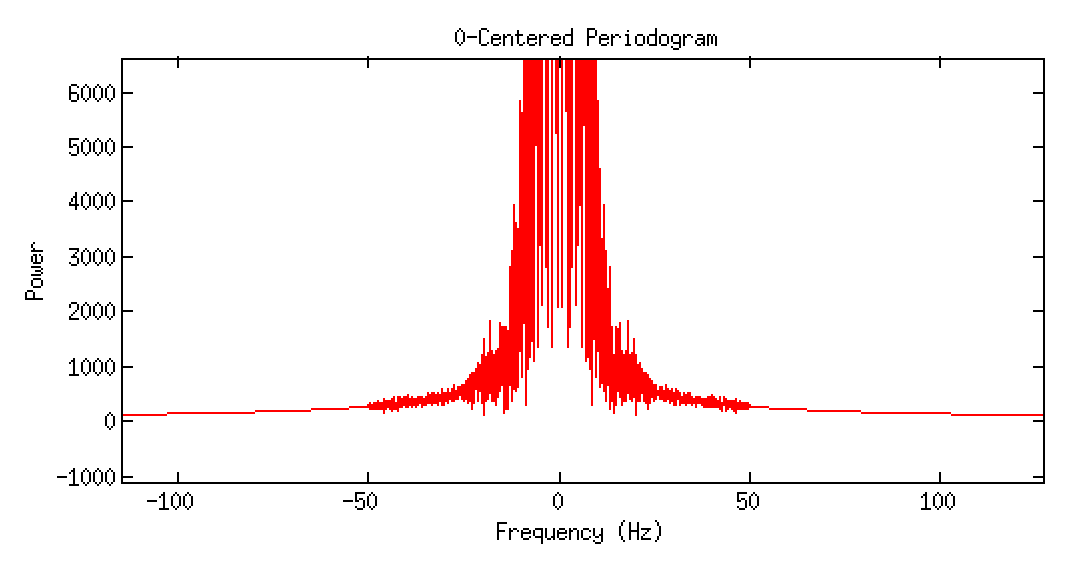
\includegraphics[width=0.7\textwidth]{freqspecafter}}
    \caption{The pulse waveform after power noise removal}
    \label{fig:afterpower}
\end{figure}

\section{Removal of pulse waveform baseline wander}
Although the collecting system the paper uses is linear-bandwidth
within [0.05Hz, 100Hz], the pulse waveform is yet interference by the
breathing and body movement during pulse capture. Otherwise, the pulse
signal of a healthy person will stay on a horizontal line, i.e. each
starting point of a pulse cycle lies on this horizontal line. See Figure~\ref{fig:baselinedrift}. As
similar to electrocardiogram (ECG) signal, the line is also called
\emph{baseline} in this paper. The baseline will bring waveform
distortion to feature extraction so as to affect the succeeding
analysis.~\cite{li1999study,allen2000variability} 
\begin{figure}[htbp]
    \begin{center}
        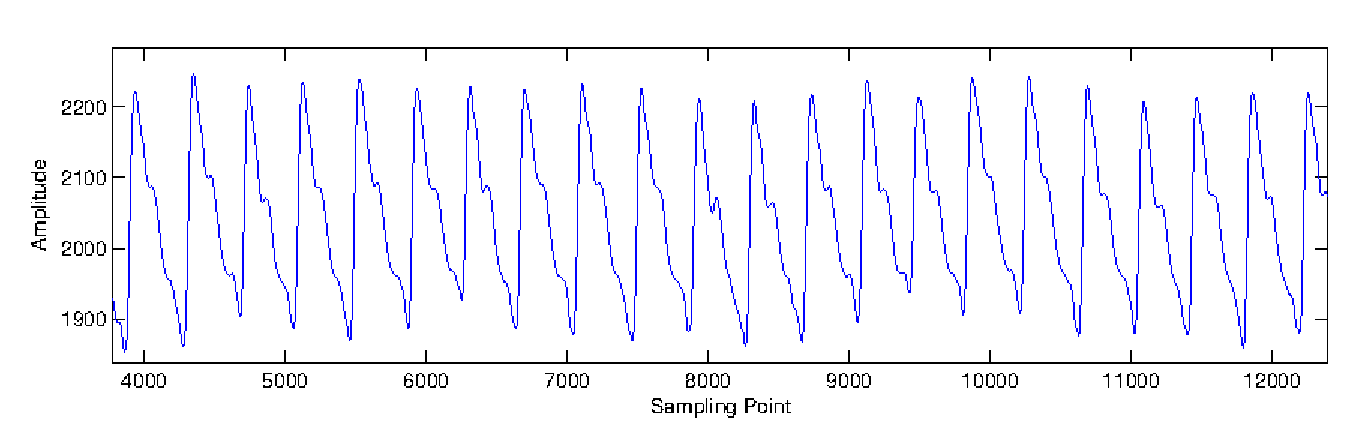
\includegraphics[width=0.8\textwidth]{baselinedrift}
    \end{center}
    \caption{The pulse wave with baseline drift}
    \label{fig:baselinedrift}
\end{figure}

The baseline wander issue has existed in physiological signal (e.g.
ECG) in a long time and many methods have been put forward in previous
work. These methods involves ensemble average, polynomial interpolation,
zero-phase filtering, morphological filtering, time-varying filtering,
adaptive filtering, wavelet-based filtering etc. All of them have
their specific applicable conditions. With the improvement of pulse
collecting system and the carefulness in actual mechanical process,
the quality of most pulse waveforms are remarkable with less severity
of baseline wander. Cubic spline interpolation is a simple but
effective approach to estimate the hidden baseline. Therefore, the
paper adopts it to remove baseline wander. 

\subsection{Starting point detecting technique}
\label{sec:startpoint}

Before beginning with the cubic spline interpolation approach, we
should detect where the starting point of each cycle is. To avoid
controversy, the \emph{starting point} in the paper prescribes the
nadir in the ascending limb. The paper employs a concept of
\emph{sliding window}. In detail, because the sampling frequency is
500Hz while the wrist pulse frequency lies in between 48Hz and 100Hz
(participants are required to calm down before collection), there must
exist at least a pulse cycle in every 500 points. The paper uses a
500 points sized window to find peaks in the whole pulse waveform. A
schematic diagram as Figure~\ref{fig:slidingwindow} can help understand. 
\begin{figure}[htpb]
    \begin{center}
        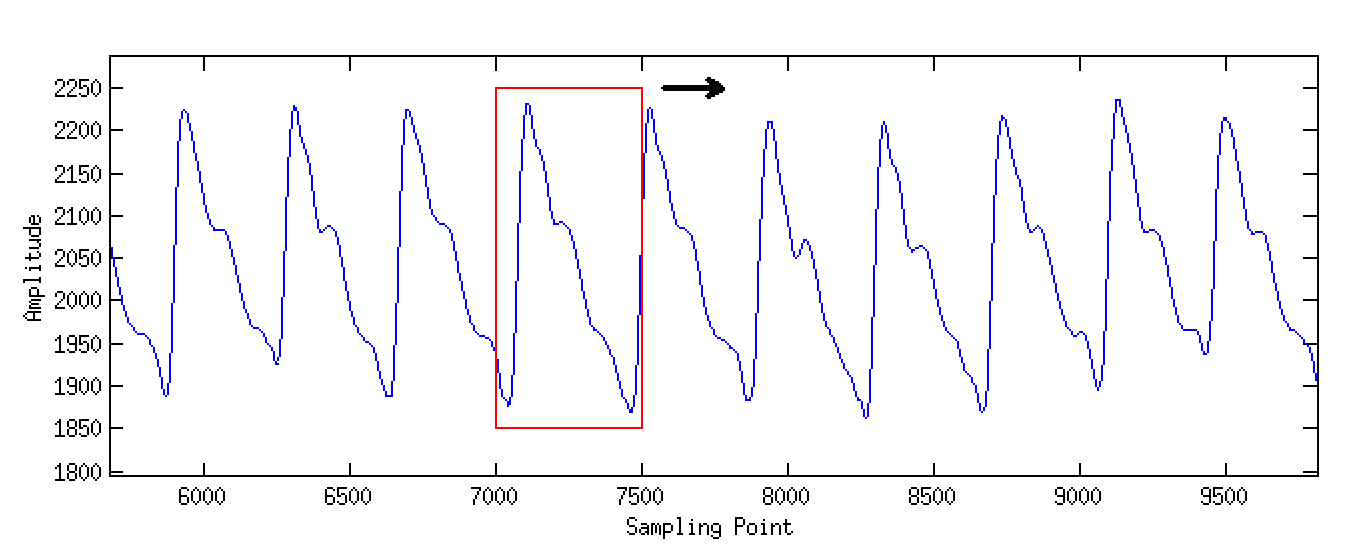
\includegraphics[width=0.7\textwidth]{slidingwindow}
    \end{center}
    \caption{The sliding window for peak detecting}
    \label{fig:slidingwindow}
\end{figure}

The peak detecting algorithm is described as follows:

\begin{algorithmic}
    \REQUIRE The denoised pulse waveform
    \ENSURE The peaks detected
    \STATE set window size as 500 points
    \FOR {each point $i$ from left to right}
        \STATE the window is the nearest 500 points centered on $i$
        \STATE find the maximum point in the window 
        \IF {the maximum point is current point $i$}
            \STATE mark $i$ as a peak
        \ENDIF
    \ENDFOR
\end{algorithmic}

Then, it is easy to get the starting points just by detecting the peaks of
up-down reversal pulse waveform using the algorithm above. The
practice on around 500 samples shows the robustness and accuracy of
this algorithm. See Figure~\ref{fig:startingpoint}.
\begin{figure}[htpb]
    \begin{center}
        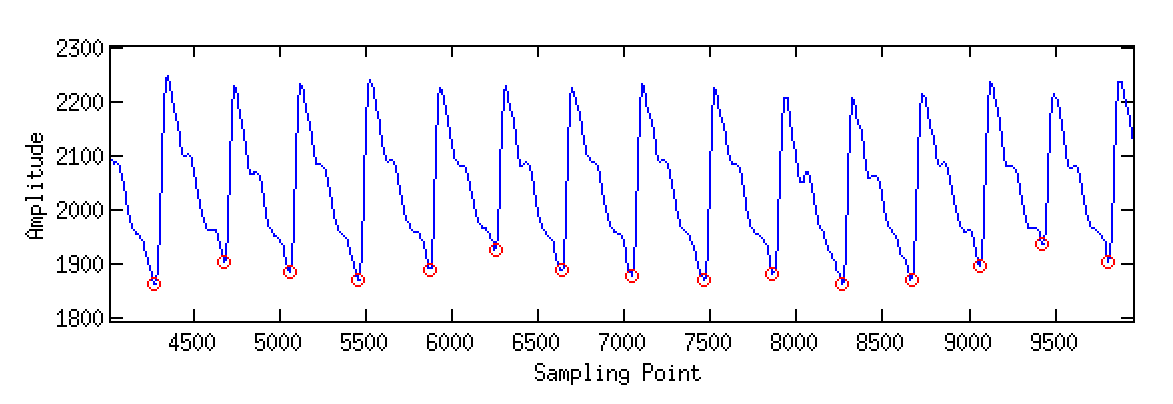
\includegraphics[width=0.7\textwidth]{startingpoint}
    \end{center}
    \caption{Starting points detected}
    \label{fig:startingpoint}
\end{figure}

\subsection{Cubic spline interpolation}
The baseline wander the breathing or body movement creates is
nonlinear and smooth, so the cubic spline interpolation could predict
the wandered baseline well. Estimation is actually a process of
function approximation. Spline interpolation is such an approximation
method to predict the major distribution from minor samples. Spline
interpolation is preferred over polynomial interpolation because the
interpolation error can be made small even when using low degree
polynomials for the spline. Spline interpolation avoids the problem of
Runge's phenomenon which occurs when interpolating between equidistant
points with high degree polynomials. 

Spline interpolation theory origins from the elastic ruler problem.
The mathematical model is described as this: The definition domain
$[a, b]$ is divided by a number of $n+1$ predefined points (the
``knots'') $(x_i, y_i)$ into small intervals $[x_i, x_{i+1}$, in
mathematical form of
$a=x_1<=\ldots<x_l=b$; The mission is to find a $n$ th-order spline
function $S(x)$ to piecewise estimate the objective function. A
piecewise cubic spline function $S(x)$ can be denoted as:
\begin{equation}
    S(x)=\sum_{k=0}^{3} a_k x^k + \sum_{i=1}{L} b_i
    (x-x_i)_{+}^{3} \quad for k=0,1,2,3; i=1,\ldots,L 
    \label{equ:cubic}
\end{equation}
\begin{equation}
    (x-x_i)_{+}^{3} = \left\{
    \begin{array}{ll}
        (x-x_i)^3, & (x \geq x_i)\\
        0, & (x<x_i)\\
    \end{array} \right.
    \label{equ:cubic2}
\end{equation}
where $a_k$ and $b_i$ denotes the polynomial coefficients and $L$
denotes the number of knots. From Equation~\ref{equ:cubic}, the
second-order differential of spline function $S(x)$ is 
\begin{equation}
    S''(x) = 2! \cdot a_2 + 3! \cdot a_3 \cdot x + 3! \cdot
    \sum_{i=1}^{L} \cdot (x-x_i)_{+}
    \label{equ:cubic3}
\end{equation}
The Equation~\ref{equ:cubic3} demonstrates that the second-order
differential in knot $(x_i, y_i)$ is continuous. Since the wandered baseline
is a continuously differentiable function, it implies that the
second-order differential of baseline is also continuous. The cubic
spline data interpolation can approach wandered baseline well. 
The Figure\ref{fig:estbaseline} and Figure~\ref{fig:baselined} respectively shows the wandered
baseline estimated and the pulse waveform after removal of baseline wander.
\begin{figure}[htpb]
    \begin{center}
        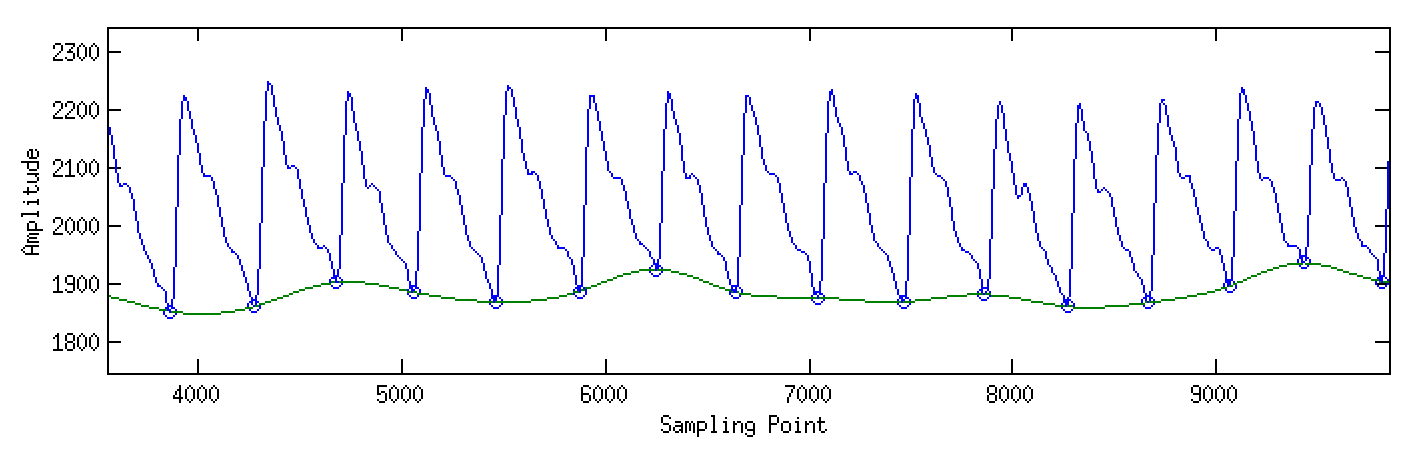
\includegraphics[width=0.7\textwidth]{cubic}
    \end{center}
    \caption{The estimated baseline wander using cubic spline interpolation}
    \label{fig:estbaseline}
\end{figure}
\begin{figure}[htpb]
    \begin{center}
        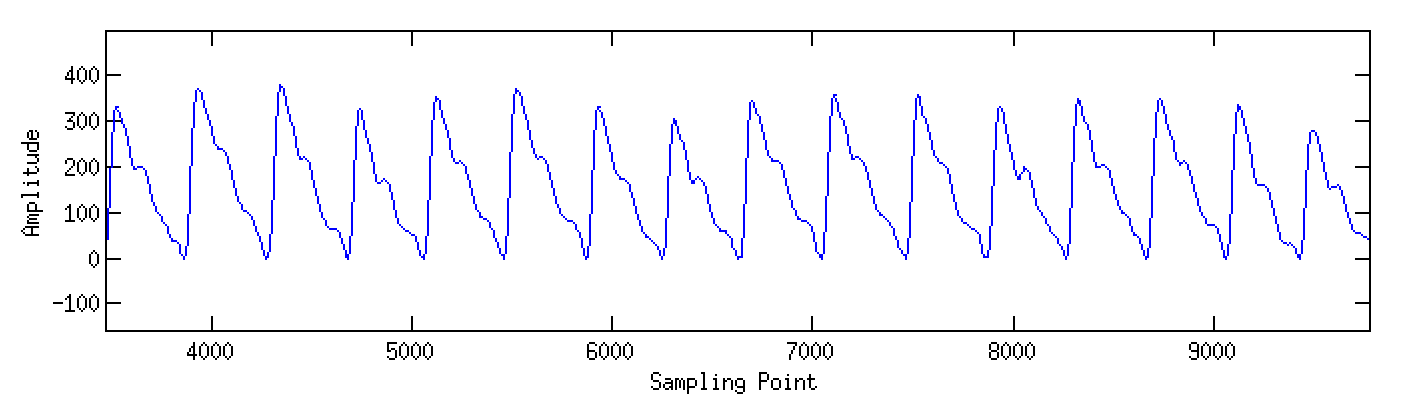
\includegraphics[width=0.7\textwidth]{baselined}
    \end{center}
    \caption{The pulse waveform after removal of baseline wander}
    \label{fig:baselined}
\end{figure}

\section{Period segmentation of pulse waveform}
The pulse image is a quasi-periodic waveforms, in which a period of
waveform records most information about wrist pulse. Beginning
with a single period pulse analysis is an effective way to understand 
in-depth meaning of pulse. The data processing in succeeding chapters
of the paper is built on a single period pulse waveform. So the
foregoing preprocessed pulse must split into single periods. 

The period segmentation, as implied by the name, is to find the starting
point and the end point. The end point is also the starting point of
next period. So only starting points are necessary to find out.
Remember the Section~\ref{sec:startpoint} introduced an algorithm
detecting the starting points. The task of period segmentation comes
much easier with the algorithm. Find two adjacent starting points
randomly and extract the period between these two points.

\section{Normalization of pulse waveform }
Because of the diversity of collecting environment and the individual
differences, the pulse may differ remarkably in amplitude. To treat them
as equal, the paper will take measures to normalize the preprocessed single
period pulse wave. Let $x$ denote a small segment signal and 
$y$ denote the normalized signal,  the
linear normalization formula is given as:
\begin{equation}
    y = \frac{x-max(x)}{max(x)-min(x)}
    \label{equ:normalize}
\end{equation}
where $max,min$ are operations to extract the maximum and the minimum,
respectively. A typical single period signal after denoising
, baseline removal and normalization pre-processing is displayed as
Figure~\ref{fig:normalize}.
\begin{figure}[htpb]
    \begin{center}
        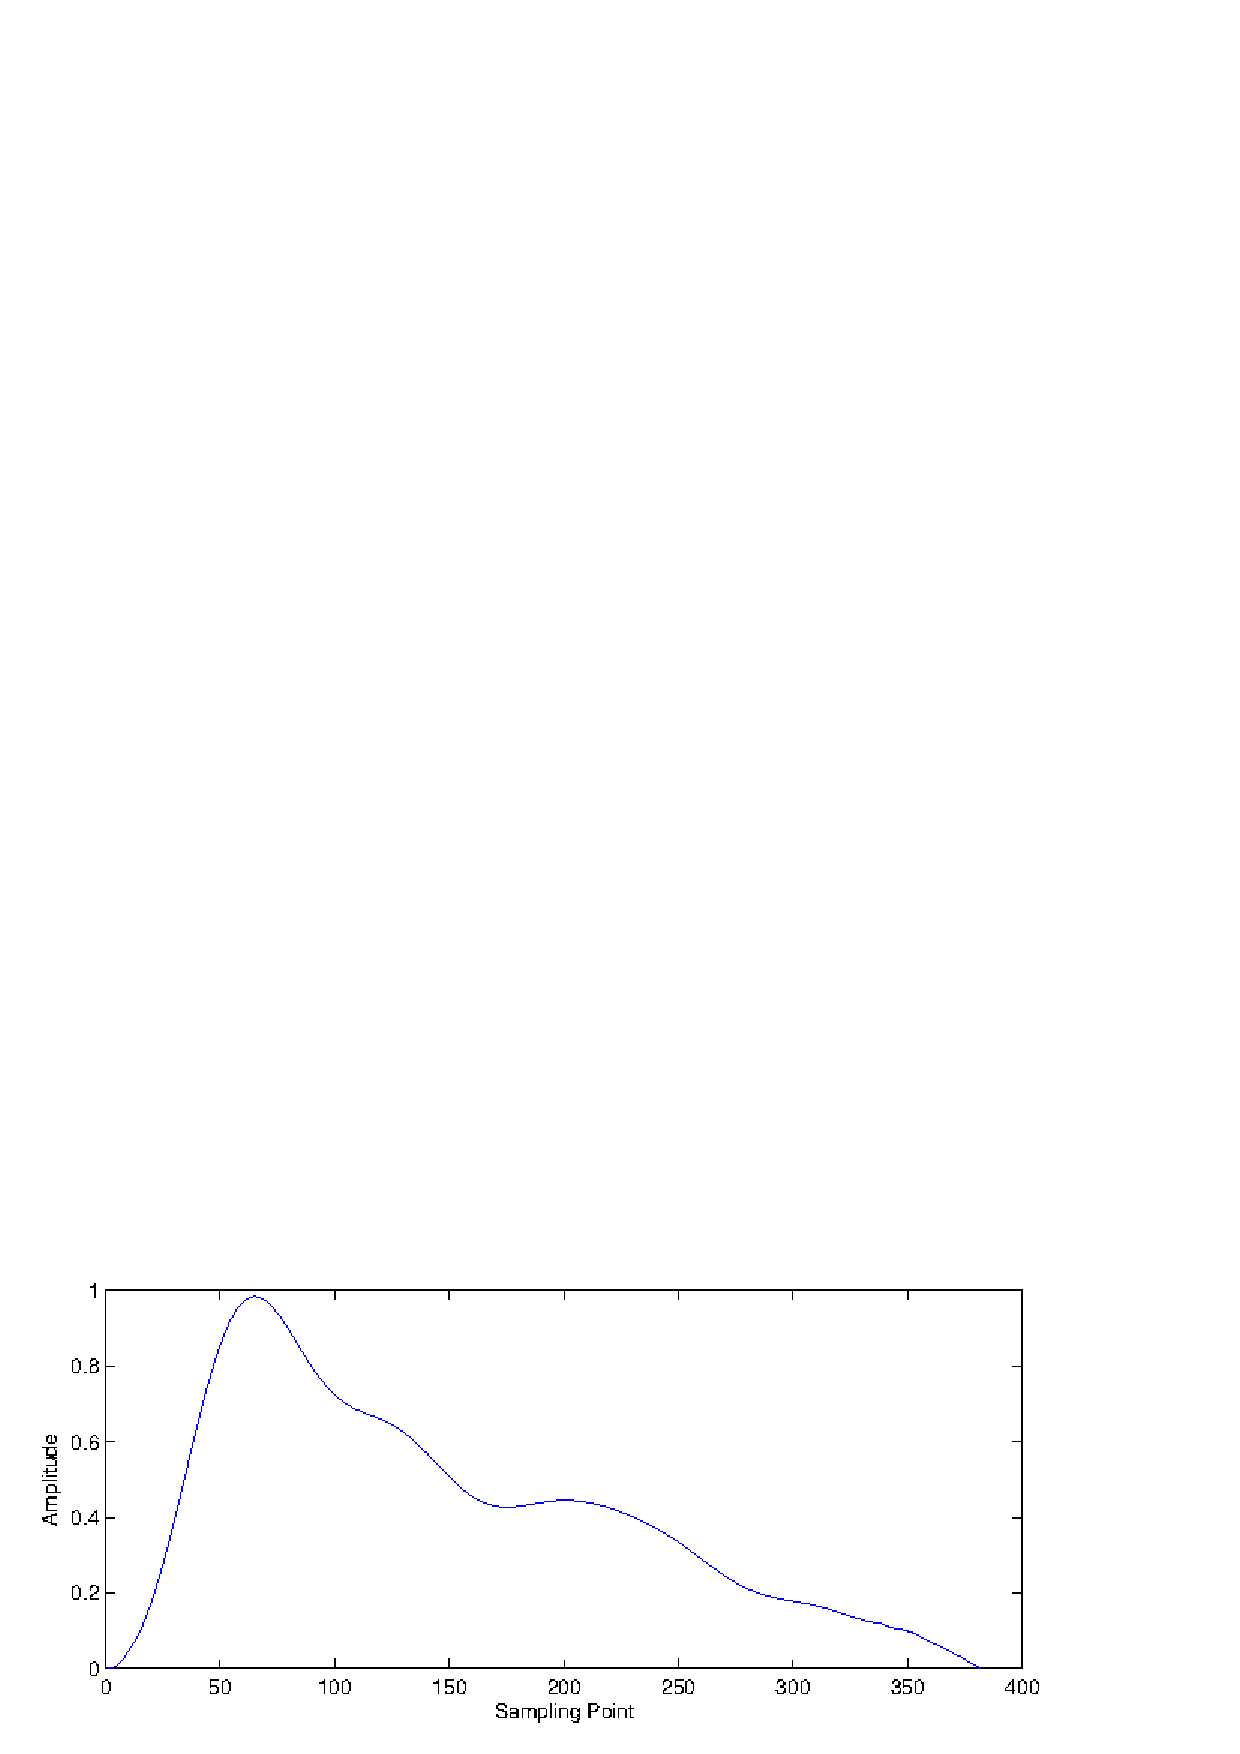
\includegraphics[width=0.7\textwidth]{normalized}
    \end{center}
    \caption{The normalized pulse signal}
    \label{fig:normalize}
\end{figure}


\section{Summary}
The chapter pre-processes the original pulse signal as needed,
including burring, baseline wander removal, segmentation and
normalization. First, the paper adopts \emph{sym8} wavelet tool and
digital linear filter to remove the high frequency noise. Second,
the simple but effective cubic spline interpolation method is applied to solve the baseline
drift issue. Finally, the optimized pulse waveform is separated into
independent periods and normalized. The single period pulse waveform
is the real input for the following chapters. 

